\clearpage
\setcounter{table}{0}
\renewcommand{\thetable}{A\arabic{table}}
\setcounter{figure}{0}
\renewcommand{\thefigure}{A\arabic{figure}}

\section*{Appendix}
\addcontentsline{toc}{section}{Appendix}

\section{Data Construction Details}\label{app:data}

\paragraph{Source and scope.} The CoreLogic Owner Transfer file compiles
recorded deeds from county recorder offices in all fifty states and the
District of Columbia. Our extract contains all record types---deeds of sale,
quitclaims, intra-family conveyances, trust transfers, and foreclosure
instruments. Coverage density is stable from 2007 onward; recording lags
truncate the file around August 2024. All annual statistics use 2007--2023;
the Proposition 19 cohort analyses use outcome windows that close by June 30,
2024.

\paragraph{Deduplication.} Multi-parcel transactions and re-recorded
corrections generate multiple rows per economic event. We keep one record per
parcel-date pair, preferring arm's-length category records and, within
category, the highest recorded consideration.

\paragraph{Classification.} The taxonomy in Section~\ref{sec:data} is
implemented with the recorder-derived interfamily indicator, the
arm's-length category code, deed type, recorded consideration, and
string features of the buyer and seller name fields (surname equality;
exact same-person matches on either buyer slot, which define the
same-person retitle class; trust keywords; estate, executor, probate, and
administrator keywords).
Name fields are populated for the large majority of records (the seller
surname is non-missing for 84 percent of interfamily events and the buyer
surname for 66 percent); missing names can only push true family transfers
into the ``other interfamily'' class, never into the market class, so the
same-surname series is a strict lower bound on inter-person family transfers.

\paragraph{Absentee recipients.} A recipient is absentee when the buyer
mailing ZIP on the deed differs from the property's situs ZIP, among records
where both are observed (77 percent of events in 2007, rising to 98 percent
by 2023). Within-state comparisons are unaffected by the secular improvement
in coverage; difference-in-differences designs absorb it in time effects.

\section{Robustness Checks}\label{app:robustness}

\paragraph{Trust-inclusive volume DiD.} Re-estimating the Proposition 19
volume difference-in-differences with trust self-transfers included in the
family aggregate yields a CA $\times$ Post coefficient of $-0.241$
(s.e.\ $0.027$), a 21 percent decline, confirming that the steady-state drop
in family transfers is not an artifact of reclassification between direct
family deeds and trust vehicles.

\paragraph{Synthetic-control in-space placebo.} The main-text inference for the
steady-state decline assigns the treatment to each donor state in turn and ranks
California's post/pre mean squared prediction error ratio in the resulting
distribution; California is second of fifty-one (Figure~\ref{fig:scm_mspe},
exact randomization $p = 0.039$).

\begin{figure}[!ht]
  \centering
  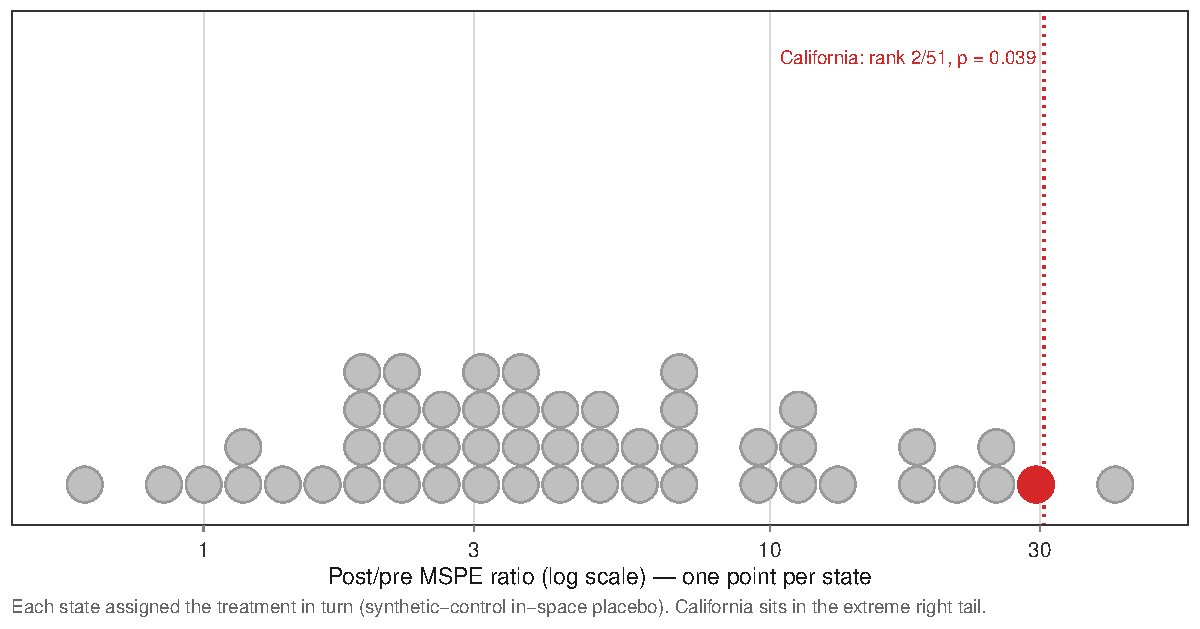
\includegraphics[width=0.82\linewidth]{figures/F7_scm_mspe_ratio.pdf}
  \caption{Synthetic-control in-space placebo: the post/pre mean squared
  prediction error ratio for each state assigned the treatment in turn.
  California (red) is second of fifty-one ($p=0.039$).}
  \label{fig:scm_mspe}
\end{figure}

\paragraph{Permutation and pre-fit-adjusted ranks.} As transparent alternatives
to the synthetic control, each donor state is assigned the treatment in turn,
each design is re-estimated, and California's coefficient is ranked in the
placebo distribution. For the annual
family-volume DiD, California ranks 5th of 51 ($p = 0.098$); for the
placebo-netted estimate, 9th ($p = 0.176$). The monthly counterfactual also
reports ranks after scaling each state's policy-window gap by its own
2018m1--2020m10 RMSPE. Under the 2019 same-month baseline, California ranks
3rd of 51 in raw anticipation, February, and 2022--2023 gaps ($p = 0.059$),
but 1st of 51 after pre-fit scaling in all three windows ($p = 0.020$). Using
a 2018--2019 same-month baseline leaves the pre-fit-adjusted ranks unchanged.
For the sold-within-24-months triple difference, $p = 0.67$; for the
estate/trust-seller market-sale DiD, $p = 0.71$ (levels) and $p = 0.63$ (net
of overall market).

\begin{figure}[!ht]
  \centering
  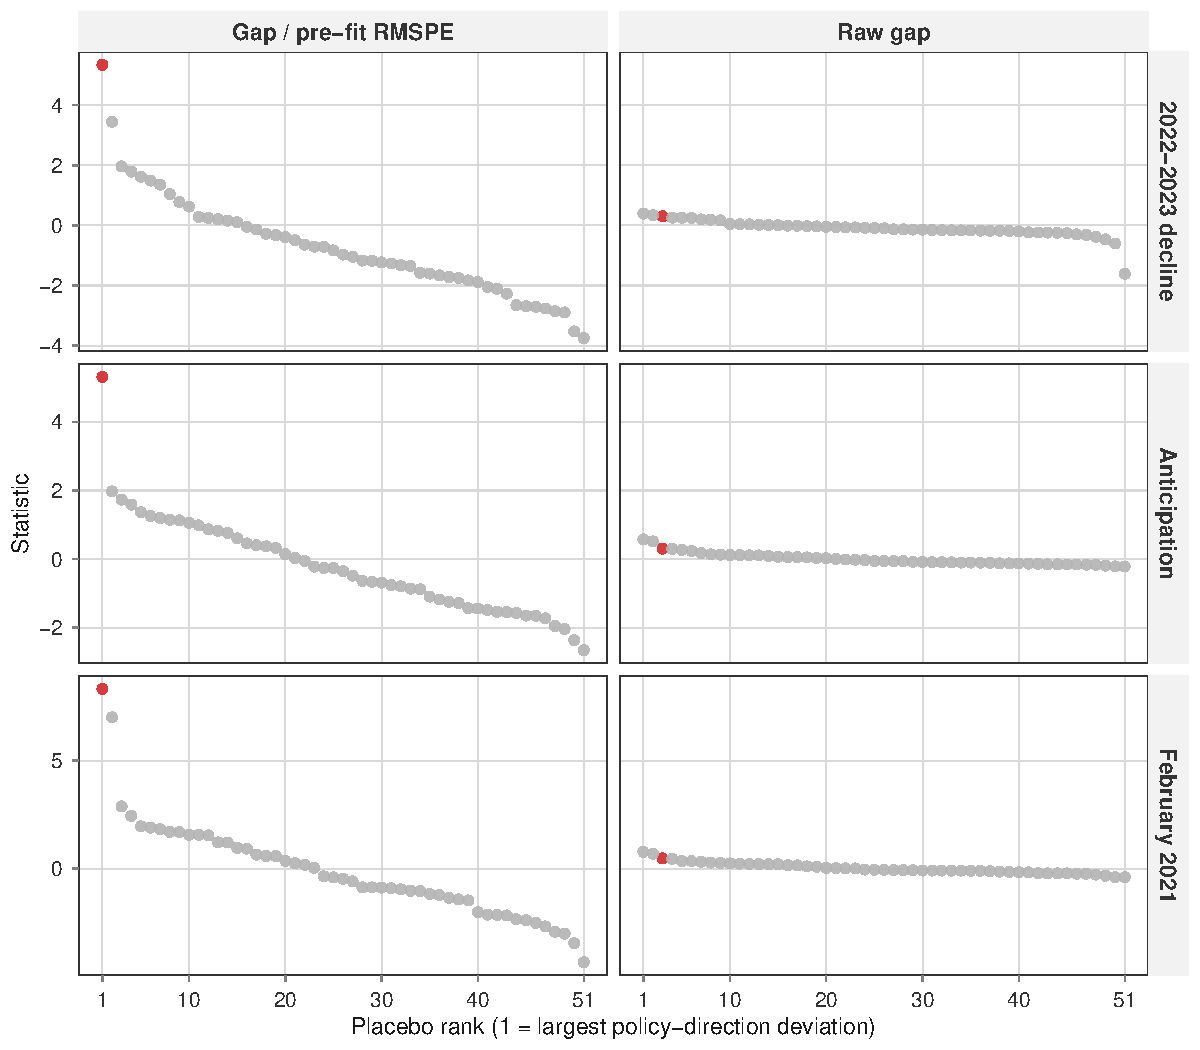
\includegraphics[width=0.92\linewidth]{figures/F7_prop19_placebo_ranks.pdf}
  \caption{Placebo ranks for the monthly Proposition~19 counterfactual. Red
  points mark California; gray points assign the same policy window to each
  donor state in turn. Raw gaps rank California third in the baseline
  comparison, while gap divided by pre-period RMSPE ranks California first.}
  \label{fig:placebo_ranks}
\end{figure}

\paragraph{Selection: sold within 24 months by cohort.} Figure~\ref{fig:sold24_cohorts}
plots the conditional-margin series discussed in Section~\ref{sec:prop19}; it is
relegated here because the triple difference is statistically unremarkable
($p = 0.67$) and the identified action is on the volume margin.

\begin{figure}[!ht]
  \centering
  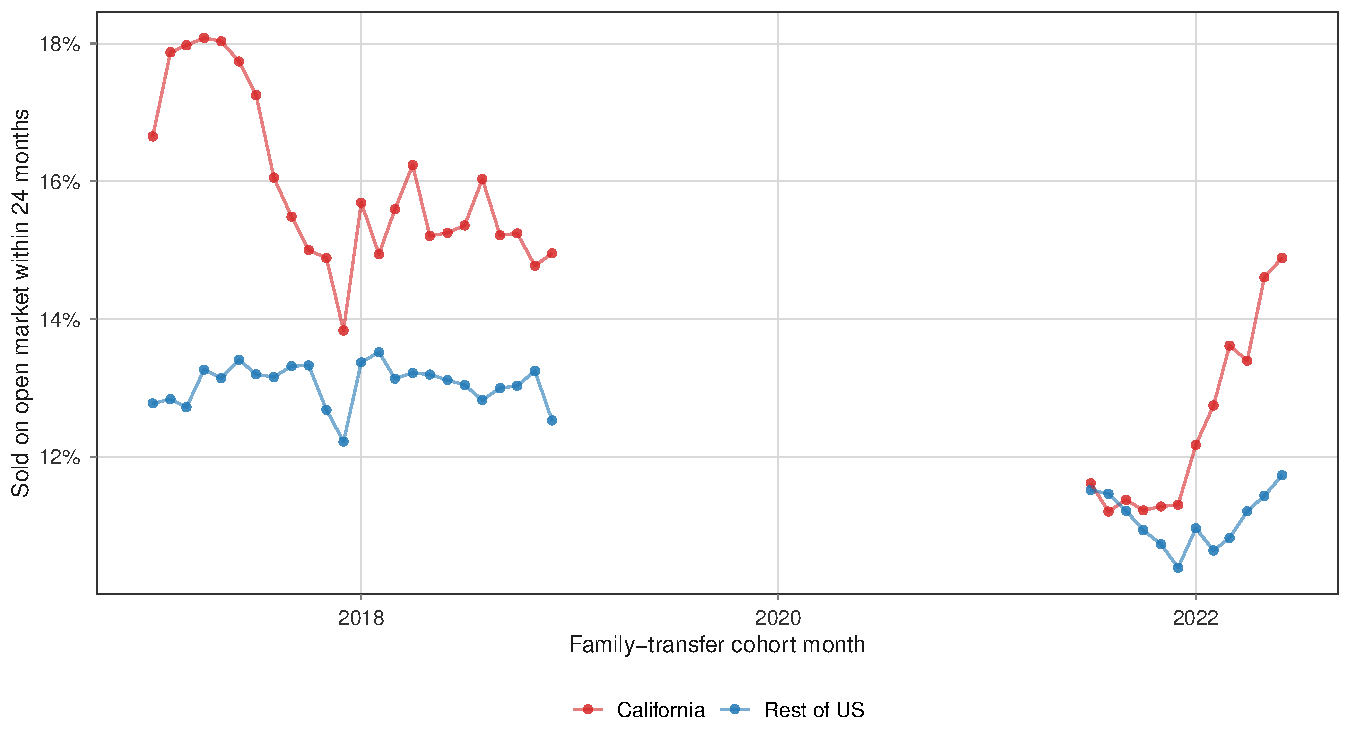
\includegraphics[width=0.85\linewidth]{figures/F5_sold24_cohorts.pdf}
  \caption{Share of family-transferred homes sold on the open market within
  24 months, by cohort month. The plotted windows exclude the transition
  period around Proposition~19; lines are not connected across the omitted
  gap.}
  \label{fig:sold24_cohorts}
\end{figure}

\paragraph{Raw difference-in-differences means.} Table~\ref{tab:raw22}
reports the unadjusted means underlying the sold-within-24-months estimates.

\begin{table}[!ht]\centering
\caption{Sold on open market within 24 months: raw cohort means}
\label{tab:raw22}
{\small
\begin{tabular}{llrrr}
\toprule
Cohort group & Region & Pre (2017m1--2018m12) & Post (2021m7--2022m6) & Change \\
\midrule
Family transfer & California & 16.1\% \; (n=470{,}163) & 12.3\% \; (n=247{,}417) & $-3.8$pp \\
Family transfer & Rest of US & 13.1\% \; (n=1{,}793{,}673) & 11.1\% \; (n=1{,}118{,}028) & $-2.0$pp \\
Market purchase & California & 6.2\% \; (n=788{,}627) & 4.7\% \; (n=421{,}807) & $-1.5$pp \\
Market purchase & Rest of US & 6.9\% \; (n=7{,}722{,}553) & 6.5\% \; (n=4{,}495{,}875) & $-0.4$pp \\
\bottomrule
\end{tabular}}
\begin{minipage}{0.95\textwidth}\vspace{2pt}{\scriptsize \textit{Notes:}
Non-corporate recipients only. Family transfer = same-surname,
cross-surname interfamily, and estate/executor classes (same-person retitles
excluded). The difference-in-differences for family transfers is $-1.8$pp;
for market purchases, $-1.1$pp; the triple difference is $-0.74$pp
(regression counterpart in Table~\ref{tab:prop19}; permutation $p = 0.67$).}\end{minipage}
\end{table}
